\documentclass[twocolumn]{svjour3-dummy}

\usepackage{xspace}
\usepackage{url}
\usepackage{cite}
\usepackage[T1]{fontenc}
\usepackage{bbm,mathtools,amssymb,bbold}
\usepackage[heavycircles]{stmaryrd}
\usepackage{paralist}
\usepackage{wrapfig}
\usepackage{tikz}
\usetikzlibrary{decorations}
\usetikzlibrary{automata}
\usetikzlibrary{shapes.multipart}
\usetikzlibrary{arrows}
\tikzset{may/.style={dashed,->,auto},
    must/.style={->,auto},
    multimust/.style={-},
    process/.style={inner sep=1.2pt,outer sep=3pt,circle,fill,draw,on grid},
    fork/.style={inner sep=0pt,outer sep=0pt,on grid}
}

\newcommand{\edgelabel}[1]{\ensuremath{\mathsf{#1}}}
\newcommand{\money}{\edgelabel{money}}
\newcommand{\extras}{\edgelabel{extras}}
\newcommand{\beverage}{\edgelabel{beverage}}
\newcommand{\onedollar}{\edgelabel{\2}}
\newcommand{\tee}{\edgelabel{tea}}
\newcommand{\coffee}{\edgelabel{coffee}}
\newcommand{\beer}{\edgelabel{beer}}
\newcommand{\milk}{\edgelabel{milk}}
\newcommand{\sugar}{\edgelabel{sugar}}
\newcommand*\labpre{\preccurlyeq}
\newcommand*\req{\textsf{req}}
\newcommand*\grant{\textsf{grant}}
\newcommand*\idle{\textsf{idle}}
\newcommand*\work{\textsf{work}}
\newcommand*\ie{\textit{i.e.},}
\newcommand*\cf{\textit{cf.}\xspace}
\newcommand*\eg{\textit{e.g.},}
\newcommand*\datop[2]{\genfrac{}{}{0pt}{0}{#1}{#2}}
\newcommand*\tatop[2]{\genfrac{}{}{0pt}{1}{#1}{#2}}
\newcommand*\impl[1]{\llbracket #1\rrbracket}
\newcommand*\Real{\mathbbm{R}}
\newcommand*\oland{\owedge}
\newcommand*\parto{\rightharpoonup}
\newcommand*\obarplus{\mathbin{\overset{\scriptscriptstyle +}{\raisebox{0pt}[1.1ex][0pt]{}}}}
\newcommand*\obarmax{\mathbin{\overset{\makebox[0pt]{}}{\raisebox{0pt}[1.05ex][0pt]{}}}}
\newcommand*\cI{\mathcal I}
\newcommand*{\must}[1]{\overset{#1}{\longrightarrow}}
\newcommand*{\omust}{\mathord{\must{}}}
\newcommand*\cD{\mathcal D}
\newcommand*{\may}[1]{\overset{#1}{\dashrightarrow}}
\newcommand*{\omay}{\mathord{\may{}}}
\newcommand*\NAA{NAA\xspace}
\newcommand*\mr{\le_\textup{\textsf{m}}}
\newcommand*\mreq{\equiv_\textup{\textsf{m}}}
\newcommand*\tr{\le_\textup{\textsf{th}}}
\newcommand*\noproof{\qed}
\newcommand*\cA{\mathcal A}
\newcommand*\Tran{\textup{\textrm{Tran}}}
\newcommand*\db{\textit{da}} \newcommand*\bd{\textit{ad}} \newcommand*\bigmid{\mathrel{\big|}}
\newcommand*\HML{\mathcal{H}}
\newcommand*\ttt{\mathbf{t\!t}}
\newcommand*\fff{\mathbf{ff}}
\newcommand*\cN{\mathcal N}
\newcommand*\lsem[1]{\llparenthesis #1\rrparenthesis}
\newcommand*\IMPL{\mathrel{\Longrightarrow}}
\newcommand*\sem[1]{\llbracket #1\rrbracket}
\newcommand*\bigland{\bigwedge}
\newcommand*\biglor{\bigvee}
\newcommand*\ddh{\textit{dn}} \newcommand*\hd{\textit{nd}} \newcommand*\viz{\textit{viz.}\xspace}
\newcommand*\cS{\mathcal S}
\newcommand*\by{/}
\newcommand*\PermL{\textit{pl}}
\newcommand*\postra[2][]{\textit{pt}_{#1}(#2)}
\newcommand*\send{\textsf{send}}
\newcommand*\early{\textsf{early}}
\newcommand*\late{\textsf{late}}
\newcommand*\LL{\mathbbm L}
\newcommand*\Realnn{\Real_{ \ge 0}}
\newcommand*\eval{\textup{\textsf{eval}}}
\newcommand*\td{d_\textup{\textsf{tr}}} \newcommand*\tdl{\td^\LL}
\newcommand*\id{\textup{\textsf{id}}}
\newcommand*\Nat{\mathbbm{N}}
\newcommand*\md{d_\textup{\textsf{m}}} \newcommand*\mdl{\smash{\md^\LL}}
\newcommand*\thd{d_\textup{\textsf{th}}} \newcommand*\thdl{\thd^\LL}



\title{Compositionality for Quantitative Specifications\thanks{This paper is based on the conference
    contribution~\cite{DBLP:conf/facs2/FahrenbergKLT14}, which has been
    presented at the 11th International Symposium on Formal Aspects of
    Component Software in Bertinoro, Italy.}}

\author{Uli Fahrenberg \and Jan K{\v r}et{\'\i}nsk{\'y} \and
  Axel Legay \and Louis-Marie Traonouez}

\institute{Uli Fahrenberg \and Axel Legay \and Louis-Marie Traonouez
  \at Irisa / Inria Rennes \and Jan K{\v r}et{\'\i}nsk{\'y} \at
  Technical University of Munich}

\begin{document}

\maketitle

\begin{abstract}
  We provide a framework for compositional and iterative design and
  verification of systems with quantitative information, such as
  rewards, time or energy. It is based on disjunctive modal transition
  systems where we allow actions to bear various types of quantitative
  information. Throughout the design process the actions can be further
  refined and the information made more precise. We show how to compute
  the results of standard operations on the systems, including the
  quotient (residual), which has not been previously considered for
  quantitative non-deterministic systems. Our quantitative framework has
  close connections to the modal nu-calculus and is compositional with
  respect to general notions of distances between systems and the
  standard operations.
\end{abstract}

\section{Introduction}
\label{sec:intro}

Specifications of systems come in two main flavors. \emph{Logical}
specifications are formalized as formulae of modal or temporal logics,
such as the modal -calculus or LTL. A common way to verify them on
a system is to translate them to automata and then analyze the
composition of the system and the automaton. In contrast, in the
\emph{behavioral} approach, specifications are given, from the very
beginning, in an automata-like formalism. Such properties can be
verified using various equivalences and preorders, such as bisimilarity
or refinement.  Here we focus on the latter approach, but also show
connections between the two.

Behavioral formalisms are particularly apt for com\-ponent-based design.
Indeed, specifications can be easily composed as well as separately
refined into more concrete ones.  The behavioral formalisms we work with
here are \emph{modal transition systems}
(MTS)~\cite{DBLP:conf/lics/LarsenT88} and their extensions. MTS are like
automata, but with two types of transitions: \emph{must}-transitions
represent behavior that has to be present in every implementation;
\emph{may}-tran\-sitions represent behavior that is allowed, but not
required to be implemented.

\begin{figure}
  \centering
  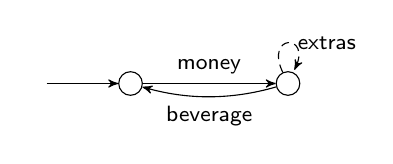
\begin{tikzpicture}[->, >=stealth', font=\footnotesize, xscale=2, yscale=1,
    state/.style={shape=circle, draw, initial text=,inner
      sep=.5mm,minimum size=3mm}]
    \node[state,initial,label=below:] (XX) at(-3,0) {};
    \node[state] (YY) at (-2,0) {};
    \path[->] (XX) edge node[above]{\money} (YY); 
    \path[densely dashed,->] (YY) edge[loop above] node[right]{\extras} (YY);
    \path[->] (YY) edge[bend left] node[below]{\beverage} (XX);
  \end{tikzpicture}
  \caption{\label{fi:vendingmachine1}
    Specification of a simple vending machine}
\end{figure}

A simple example of a vending machine specification, in
Fig.~\ref{fi:vendingmachine1}, describes that any correct implementation
must be ready to accept \money, then may offer the customer to choose
\extras\ and must issue a \beverage. While the must-transitions are
preserved in the refinement process, the may-transitions can be either
implemented and turned into must-transitions, or dropped.

\begin{figure}\centering
  \begin{tikzpicture}[->, >=stealth', font=\footnotesize, xscale=2, yscale=1,
    state/.style={shape=circle, draw, initial text=,inner
      sep=.5mm,minimum size=3mm}]
    \node[state,initial,label=below left:] (X) {};
    \node[state] (Y1) at (0,1) {};
    \node[state] (Y2) at (1,0) {};
    \node[state] (Z1) at (2,1) {};
    \node[state] (Z2) at (2,-1) {};
    \path (X) edge node[right,pos=0.9]{\onedollar} (Y1)
    (X) edge node[above,pos=0.8]{\twodollar} (Y2)
    (Y1) edge[out=210, in=120, looseness=1] node[left]{\tee} (X)
    (Y1) edge[out=180, in=150, looseness=2] node[left]{\coffee} (X)
    (Y2) edge[bend left] node[below,pos=0.3]{\beer} (X)
    (Y2) edge[] node[right]{\milk} (Z1)
    (Z1) edge[loop above, densely dashed] node[right]{\sugar} (Z1)
    (Y2) edge[] node[right]{\sugar} (Z2)
    (Z2) edge[bend left] node[below]{\tee} (X)
    (Z2) edge[out=210,in=270,looseness=1.3] node[below]{\coffee} (X)
    (Z1) edge[bend right] node[below,pos=.4]{\tee} (X)
    (Z1) edge[out=150,in=60,looseness=1.3] node[above]{\coffee} (X)
    ;
  \end{tikzpicture}
  \caption{\label{fi:vendingmachine}
    Specification of another vending machine}
\end{figure}

This low-level refinement process is, however, insufficient when the
designer wants to get more specific about the implemented actions, such
as going from the coarse specification just described to the more
fine-grained specification of Fig.~\ref{fi:vendingmachine}.  In order to
relate such specifications, MTS with \emph{structured labels} have been
introduced \cite{DBLP:journals/mscs/BauerJLLS12}. Given a preorder on
labels, relating for instance , we can refine a
transition label into one which is below, for example implement
``\beverage'' with its refinement ``\coffee''.

\begin{figure}
  \centering
  \begin{tikzpicture}[->, >=stealth', font=\footnotesize,
    state/.style={shape=circle, draw, initial text=,inner
      sep=.5mm,minimum size=2mm}, scale=1.4]
    \begin{scope}
      \node[state,initial,label=below left:] (X) {};
      \node[state] (Y) at (2,0) {};
      \path[densely dashed,->] (X) edge node[above]{} (Y); 
      \path[densely dashed,->] (X) edge[loop above]
      node[above]{} (X);
      \path (Y) edge[bend left] node[below]{} (X);
    \end{scope}
  \end{tikzpicture}
  \caption{\label{fi:realtimeexint}
    A simple real-time specification}
\end{figure}

This framework can be applied to various preorders. For example, one can
use labels with a discrete component carrying the action information and
an interval component to model time duration or energy consumption.  As
an example, consider the simple real-time property in
Fig.~\ref{fi:realtimeexint}: ``after a \req(uest), \grant\ has to be
executed within  time units without the process being 
meanwhile''. The transition  could be safely refined to
 for any .

We proceed to identify several shortcomings of the current approaches.

\paragraph{Expressive power.} 

The current theory of structured
labels~\cite{DBLP:journals/mscs/BauerJLLS12,
  DBLP:journals/acta/FahrenbergL14} is available only for the basic
MTS. Very often one needs to use richer structures such as
\emph{disjunctive} MTS (DMTS)~\cite{DBLP:conf/lics/LarsenX90,
  DBLP:conf/atva/BenesCK11} or acceptance
automata~\cite{report/irisa/Raclet07,
  DBLP:journals/jacm/Hennessy85}. While MTS generally cannot express
disjunction of properties, DMTS and further related formalisms can and
are, in fact, equivalent to the modal
-calculus~\cite{DBLP:conf/concur/BenesDFKL13,
  DBLP:conf/ictac/FahrenbergLT14}, \ie~the maximal-fixed point
fragment of the modal -calculus~\cite{DBLP:journals/tcs/Kozen83}.

\begin{figure}
  \centering
  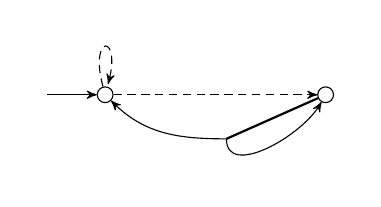
\begin{tikzpicture}[->, >=stealth', font=\footnotesize,
    state/.style={shape=circle, draw, initial text=,inner
      sep=.5mm,minimum size=2mm}, scale=1.4]
    \begin{scope}
      \node[state,initial,label=below left:] (X) {};
      \node[state, label=right:] (Y) at (2,0) {};
      \path[densely dashed,->] (X) edge node[above]{} (Y); 
      \path[densely dashed,->] (X) edge[loop above]
      node[above]{} (X);
      \coordinate (Yd) at (1.1,-.4) {};
      \path (Y) edge[-, thick] (Yd);
      \path (Yd) edge[out= 180, in= -45] node[below]{} (X);
      \path (Yd) edge[out= -90, in= 240] node[right,
      pos=0.5]{~~~} (Y);
    \end{scope}
  \end{tikzpicture}
  \caption{\label{fi:quantspecex1}
    A disjunctive modal transition system}
\end{figure}

\begin{figure}\centering
  
  \caption{\label{fi:quantspecex}
    The -calculus translation of the DMTS in
    Fig.~\ref{fi:quantspecex1}}
\end{figure}

This allows, for instance, to prohibit deadlocks as in the example in
Fig.~\ref{fi:quantspecex1}. The disjunctive must, depicted as a
branching arrow, requires at least one of the transitions to be
present. Thus we allow the deadline for \grant\ to be reset if
additional \work\ is generated. Note that specifying \grant\ and
\work\ as two separate must-transitions would not allow postponing the
deadline; and two separate may-transitions would not guarantee any
progress, as none of them has to be implemented. We hence propose
\emph{DMTS with structured labels} and also extend the equivalence
between DMTS and the modal
-calculus~\cite{DBLP:conf/concur/BenesDFKL13,
  DBLP:conf/ictac/FahrenbergLT14} to our setting.
Figure~\ref{fi:quantspecex} shows a -calculus translation of the
DMTS in Fig.~\ref{fi:quantspecex1}.

\paragraph{Robustness.}

\begin{figure}
  \centering
  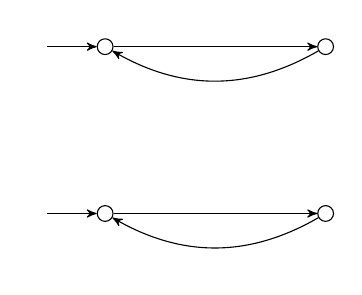
\begin{tikzpicture}[->, >=stealth', font=\footnotesize,
    state/.style={shape=circle, draw, initial text=,inner
      sep=.5mm,minimum size=2mm}, scale=1.4]
    \begin{scope}
      \node[state,initial,label=below:] (X) {};
      \node[state] (Y) at (2,0) {};
      \path (X) edge node[above]{} (Y); 
      \path (Y) edge[bend left] node[below]{} (X);
    \end{scope}
    \begin{scope}[yshift=-10ex]
      \node[state,initial,label=below:] (X) {};
      \node[state] (Y) at (2,0) {};
      \path (X) edge node[above]{} (Y); 
      \path (Y) edge[bend left] node[below]{} (X);
    \end{scope}
  \end{tikzpicture}
  \caption{\label{fi:quantimp1}
    Two implementations}
\end{figure}

Consider again the request-grant example in Fig.~\ref{fi:quantspecex1},
together with the two labeled transition systems in
Fig.~\ref{fi:quantimp1}.  While , issuing \grant\ after precisely 5
time units, is a valid implementation of , if there is but a small
positive drift in the timing, like in , it is not an implementation
anymore.  However, this drift might be easily mended or just might be
due to measuring errors.

\begin{figure}\centering
  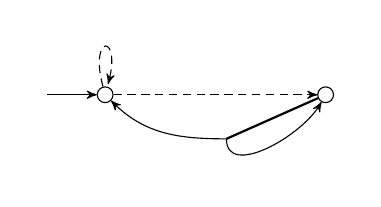
\begin{tikzpicture}[->, >=stealth', font=\footnotesize,
    state/.style={shape=circle, draw, initial text=,inner
      sep=.5mm,minimum size=2mm}, scale=1.4]
    \begin{scope}
      \node[state,initial,label=below left:] (X) {};
      \node[state, label=right:] (Y) at (2,0) {};
      \path[densely dashed,->] (X) edge node[above]{} (Y); 
      \path[densely dashed,->] (X) edge[loop above]
      node[above]{} (X);
      \coordinate (Yd) at (1.1,-.4) {};
      \path (Y) edge[-, thick] (Yd);
      \path (Yd) edge[out= 180, in= -45] node[below]{} (X);
      \path (Yd) edge[out= -90, in= 240] node[right,
      pos=0.4]{} (Y);
    \end{scope}
  \end{tikzpicture}
  \caption{\label{fi:quantimp}
    Another DMTS specification}
\end{figure}

Therefore, when models and specifications contain such quantitative
information, the standard Boolean notions of satisfaction and refinement
are of limited utility~\cite{DBLP:conf/fm/HenzingerS06,
  DBLP:journals/cejcs/Sifakis11} and should be replaced by notions which
are more robust to perturbations.  For another example, the DMTS of
Fig.~\ref{fi:quantimp} is \emph{not} a refinement of the one in
Fig.~\ref{fi:quantspecex1}, but for all practical purposes, it is rather
close.

One approach to robustness is to employ metric \emph{distances} instead
of Boolean relations; this has been done for example~in~\cite{DBLP:journals/tse/AlfaroFS09,
  DBLP:conf/mfcs/LarsenMP12, DBLP:journals/tcs/DesharnaisGJP04,
  DBLP:journals/tcs/BreugelW05, DBLP:conf/formats/HenzingerMP05,
  DBLP:journals/tcs/CernyHR12, DBLP:conf/forte/Romero-HernandezF12,
  DBLP:conf/wadt/Romero-HernandezF12, DBLP:journals/tcs/AlfaroFHMS05,
  DBLP:conf/concur/Alfaro03 } and many other papers.  An advantage of
behavioral specification formalisms is that models and specifications
are closely related, hence distances between models can easily be
extended to distances between specifications.  We have developed a
distance-based approach for MTS in~\cite{
  DBLP:conf/csr/BauerFLT12,
  DBLP:conf/mfcs/BauerFJLLT11,
  DBLP:journals/acta/FahrenbergL14, DBLP:journals/fmsd/BauerFJLLT13} and
shown in~\cite{DBLP:journals/tcs/FahrenbergL14,
  DBLP:journals/acta/FahrenbergL14,
  DBLP:conf/csr/BauerFLT12,
  DBLP:conf/fsttcs/FahrenbergLT11,
  DBLP:conf/aplas/FahrenbergL13} that a good general setting is given by
recursively specified trace distances on an abstract quantale.  Here we
extend this to DMTS.

\paragraph{Compositionality.}
The framework should be compositional. In the quantitative setting, this
in essence means that the operations we define on the systems should
behave well with respect not only to satisfaction, but also to the
distances. For instance, if  is close to  and  close to
, then also the structural composition  should be close
to . We prove this for the usual operations; in particular,
we give a construction for such a well-behaved
\emph{quotient}.

The quotient of  by  is the most general specification that, when
composed with , refines . This operation is thus useful for
computing missing parts of a system to be implemented, when we already
have several components at our disposal. The construction is complex
already in the non-quantitative
setting~\cite{DBLP:conf/concur/BenesDFKL13} and the extension of the
algorithm to structured labels is non-trivial.

\paragraph{Our contribution.}
To sum up, we extend the framework of structured labels to DMTS and
the modal -calculus.  To be able to reason about robustness, we
equip this framework with distances and give constructions for the
structured analogues of the standard operations, so that they behave
compositionally with respect to the distances.

\paragraph{Further related work.}

Refinement of components is a frequently used design approach in various
areas, ranging from subtyping~\cite{DBLP:journals/toplas/LiskovW94} over
the Java modeling language JML~\cite{DBLP:conf/fase/JacobsP01} or
correct-by-design class diagram
operations~\cite{DBLP:conf/fase/FahrenbergALW14} to interface theories
close to MTS such as interface
automata~\cite{DBLP:conf/sigsoft/AlfaroH01} based on alternating
simulation. A variant of alternating simulation called
cova\-riant-contravariant simulation has been compared to MTS modal
refinement in~\cite{DBLP:journals/scp/AcetoFFIP13}. The graphical
representability of these variants was studied
in~\cite{DBLP:journals/tcs/BoudolL92, DBLP:conf/concur/BenesDFKL13}.

Quantitative specifications have been introduced in other settings.  At
first, the focus was on probabilities~\cite{DBLP:conf/lics/HuthK97, mu2,
  DBLP:conf/fossacs/Mio11}, but later, predicates with values in
arbitrary metric spaces were also
introduced~\cite{DBLP:journals/tse/AlfaroFS09}.  Robustness of
probabilistic specifications is considered
in~\cite{DBLP:journals/tcs/AlfaroFHMS05, DBLP:journals/tse/AlfaroFS09,
  DBLP:conf/concur/Alfaro03}.  It is our hope that the close
relationship between quantitative DMTS and the quantitative modal
-calculus which we expose in this paper will aid in the development
of theory and tools also for probabilistic specifications.

There are a number of extensions of MTS specifically designed for
coping with real-time properties: the timed input-output
specifications of~\cite{DBLP:journals/sttt/DavidLLNTW15}, the timed
interfaces of~\cite{DBLP:conf/emsoft/AlfaroHS02}, and the modal
event-clock specifications of~\cite{DBLP:journals/scp/BertrandLPR12}.
Robustness for timed input-output specifications is considered
in~\cite{DBLP:journals/tcs/LarsenLTW14,
  DBLP:journals/corr/abs-1207-4269, DBLP:conf/formats/LarsenLTW11}.
With only little extra work, our notions of distances and robustness
can be applied to real-time specifications,
see~\cite{DBLP:journals/corr/abs-1207-4268} for modal event-clock
specifications.

Some other extensions of MTS have been developed for probabilistic
properties: the constraint Markov chains
of~\cite{DBLP:journals/jlp/DelahayeLLPW12,
  DBLP:journals/tcs/CaillaudDLLPW11,
  DBLP:conf/lics/JonssonL91} and the abstract probabilistic automata
of~\cite{DBLP:journals/tcs/CaillaudDLLPW11}.  Distances for such
specifications are used in~\cite{DBLP:journals/corr/abs-1212-4288}, but
no work on robustness is available.

\section{Structured Labels}
\label{se:structlabels}

Let  be a poset with partial order .  We think of
 as \emph{label refinement}, so that if , then 
is less permissive (more restricted) than .

\begin{definition}
  A label  is an \emph{implementation label} if  implies  for all .  The set of implementation
  labels is denoted , and for , we let  denote the set of its
  implementations.
\end{definition}

Hence  is an implementation label iff  cannot be further
refined.  Note that  implies 
for all .

\begin{example}
  \label{ex:labelsets}
  A trivial but important example of our label structure is the
  \emph{discrete} one in which label refinement  is equality
  (and ).  This is equivalent to the ``standard'' case
  of \emph{unstructured} labels.

  A typical label set in quantitative applications consists of a
  discrete component and real-valued weights.  For specifications,
  weights are replaced by (closed) weight \emph{intervals}, so that
   for a finite set ,
  \cf~\cite{DBLP:journals/fmsd/BauerFJLLT13,
    DBLP:journals/mscs/BauerJLLS12}.  Label refinement is given by  iff  and , so that labels are more refined if they
  specify smaller intervals; thus, .

  For a quite general setting, we can instead start with an arbitrary
  set  of implementation labels, let , the
  powerset, and  be subset
  inclusion.  Then  for all .  (Hence we
  identify implementation labels with one-element subsets of .)
  \qed
\end{example}

\subsection{Label operations}

Specification theories come equipped with several standard operations
that make compositional software design
possible~\cite{DBLP:conf/fase/BauerDHLLNW12}: conjunction for merging
viewpoints covering different system's
aspects~\cite{DBLP:conf/sigsoft/UchitelC04,
  DBLP:conf/concur/Ben-DavidCU13}, structural composition for running
components in parallel, and quotient to synthesize missing parts of
systems~\cite{DBLP:conf/lics/LarsenX90}. In order to provide them
for DMTS, we first need the respective atomic operations on their action
labels.

We hence assume that  comes equipped with a partial conjunction,
\ie~an operator  for which it
holds that
\begin{enumerate}[(1)]
\item \label{en:oland.lb} if  is defined, then  and , and
\item \label{en:oland.glb} if  and , then
   is defined and .
\end{enumerate}
Note that by these properties, any two partial conjunctions on 
have to agree on elements for which they are both defined.

\begin{example}
  \label{ex:conjunction}
  For discrete labels, the unique conjunction operator is given by
  
  Indeed, by property~\eqref{en:oland.glb},  must be
  defined for , and by~\eqref{en:oland.lb}, if  is defined, then  and .

  For labels in ,
  the unique conjunction is
  
  To see uniqueness, let  for .
  Using property~\eqref{en:oland.glb}, we see that 
  must be defined when  and , and by~\eqref{en:oland.glb}, if  is
  defined, then  and , and ,  imply .

  Finally, for the case of specification labels as sets of
  implementation labels, the unique conjunction is . \qed
\end{example}

For structural composition and quotient of specifications, we assume a
partial \emph{label synchronization} operator  which specifies how to compose
labels.  We assume  to be associative and commutative, with the
following technical property which we shall need later: For all  with  and ,
 is defined iff  is, and if both are
defined, then .

\begin{example}
  \label{ex:composition}
  For discrete labels, the conjunction of Example~\ref{ex:conjunction}
  is the same as CSP-style composition, \ie~ if  and
  undefined otherwise, but other compositions can easily be defined.

  For labels in , several
  useful label synchronization operators may be defined for different
  applications.  One is given by \emph{addition} of intervals, \ie
  
  for example modeling computation time of actions on a single
  processor.  Another operator, useful in scheduling, uses maximum
  instead of addition:
  

  For set-valued specification labels, we may take any synchronization
  operator  given on implementation labels  and lift it
  to one on  by . \qed
\end{example}

\section{Specification Formalisms}
\label{se:formalisms}

In this section we introduce the specification formalisms which we use
in the rest of the paper.  The universe of models for our specifications
is the one of standard \emph{labeled transition systems}.  For
simplicity of exposition, we work only with \emph{finite} specifications
and implementations, but most of our results extend to the infinite (but
finitely branching) case.

A \emph{labeled transition system} (LTS) is a structure  consisting of a finite set  of states, an initial state
, and a transition relation .  We usually write  instead of .  Note that transitions are labeled with
\emph{implementation} labels.

\subsection{Disjunctive Modal Transition Systems}

A \emph{disjunctive modal transition system} (DMTS) is a structure
 consisting of finite sets  of states and initial states, respectively, may-tran\-sitions
, and disjunctive
must-transitions .  It is
assumed that for all  and  there is  with .

\begin{example}
  The specification  in Fig.~\ref{fi:quantspecex} has a
  may-transition to ; from there we have a disjunctive
  must-transition with identical underlying may-transitions. The
  intuitive meaning of the transition, that either \grant\ or \work\
  must be available, is formalized below using the modal
  refinement. \qed
\end{example}

Note that we allow multiple (or zero) initial states.  We write
 instead of  and 
instead of .

A DMTS  is an \emph{implementation} if
, , and  is a singleton; DMTS
implementations are hence isomorphic to LTS.

DMTS were introduced in~\cite{DBLP:conf/lics/LarsenX90} in the context
of equation solving, or \emph{quotient} of specifications by processes
and are used \eg~in~\cite{DBLP:conf/atva/BenesCK11} for LTL model
checking.  They are a natural extension of \emph{modal} transition
systems~\cite{DBLP:conf/lics/LarsenT88}, which are DMTS in which all
disjunctive must-transitions  lead to singletons ; in fact, DMTS are the closure of MTS under
quotient~\cite{DBLP:conf/lics/LarsenX90}.

We introduce a notion of modal refinement of DMTS with structured
labels.  For discrete labels, it coincides with the classical
definition~\cite{DBLP:conf/lics/LarsenX90}.

\begin{definition}
  Let  and  be DMTS.  A relation  is
  a \emph{modal refinement} if it holds for all  that
  \begin{itemize}
  \item for all  there is 
    such that  and , and
  \item for all  there is  such that
    for all  there is  with
     and .
  \end{itemize}
   \emph{refines} , denoted , if there
  exists an \emph{initialized} modal refinement , \ie~one for which
  it holds that for every  there is  for
  which .
\end{definition}

Note that this definition reduces to the one
of~\cite{DBLP:conf/lics/LarsenX90, DBLP:conf/atva/BenesCK11} for
discrete labels (\cf~Example~\ref{ex:labelsets}).

We write  if  and .
The \emph{implementation semantics} of a DMTS  is .  This is, thus, the set of
all LTS which satisfy the specification given by the DMTS .  We say
that  \emph{thoroughly refines} , and write , if .

The below proposition, which follows directly from transitivity of modal
refinement, shows that modal refinement is \emph{sound} with respect to
thorough refinement; in the context of specification theories, this is
what one would expect.  It can be shown that modal refinement is also
\emph{complete} for \emph{deterministic}
DMTS~\cite{DBLP:journals/tcs/BenesKLS09}, but we will not need this
here.

\begin{proposition}\label{prop:mrtr}
  \label{pr:mrvstr}
  For all DMTS , ,  implies . \noproof
\end{proposition}

\subsection{Acceptance automata}

A \emph{non-deterministic acceptance automaton} (\NAA) is a structure
, with  finite sets of states and
initial states and  an assignment
of \emph{transition constraints}.
The intuition is that a transition constraint  specifies a disjunction of  choices  as to
which transitions from  have to be implemented.

An \NAA is an \emph{implementation} if  is a singleton and
it holds for all  that  is a singleton; hence \NAA implementations are
isomorphic to LTS.
Acceptance automata were first introduced
in~\cite{report/irisa/Raclet07}, based on the notion of acceptance trees
in~\cite{DBLP:journals/jacm/Hennessy85}; however, there they are
restricted to be \emph{deterministic}.  We employ no such restriction
here.

In~\cite{DBLP:conf/concur/BenesDFKL13}, translations were discovered
between DMTS and \NAA.  For a DMTS  and
, let  and
define the \NAA .
For an \NAA , define the DMTS  by


Similarly to a theorem of~\cite{DBLP:conf/concur/BenesDFKL13,
  DBLP:conf/ictac/FahrenbergLT14}, we can now show the following:

\begin{theorem}
  \label{th:dmtsvsaa-bool}
  For all DMTS ,  and \NAA , ,  iff  and  iff .  \noproof
\end{theorem}

This structural equivalence will allow us to freely translate forth and
back between DMTS and \NAA in the rest of the paper.  Note, however, that
the state spaces of  and  are not the same; the one of
 may be exponentially larger.
\cite{DBLP:conf/ictac/FahrenbergLT14}~shows that this blow-up is
unavoidable.

From a practical point of view, DMTS are a somewhat more useful
specification formalism than \NAA.  This is because they are usually more
compact and easily drawn and due to their close relation to the modal
-calculus, see below.

\subsection{The Modal -Calculus}

The modal -calculus~\cite{DBLP:journals/deds/FeuilladeP07} is the
maximal-fixed point fragment of the modal
-calculus~\cite{DBLP:journals/tcs/Kozen83}, \ie~the modal
-calculus without negation and without the minimal fixed point
operator.  This is also sometimes called \emph{Henn\-essy-Milner logic
  with maximal fixed points} and represented using equation systems in
Hennessy-Milner logic with variables,
see~\cite{DBLP:journals/tcs/Larsen90, books/AcetoILS07}.  We will use
this representation below.  In~\cite{DBLP:conf/concur/BenesDFKL13},
translations were discovered between DMTS and the modal
-calculus, and refining the translations
in~\cite{DBLP:conf/ictac/FahrenbergLT14}, we could show that for
discrete labels, these formalisms are \emph{structurally equivalent}.

For a finite set  of variables, let  be the set of
\emph{Hennessy-Milner formulae}, generated by the abstract syntax , for  and
.  A \emph{-calculus expression} is a structure , with  sets of variables and  a \emph{declaration}.

We recall the greatest fixed point semantics of -calculus
expressions from~\cite{DBLP:journals/tcs/Larsen90}, but extend it to
structured labels.  Let  be an LTS, then an
\emph{assignment} is a mapping .  The set of
assignments forms a complete lattice with order  iff  for all  and
lowest upper bound .

The semantics of a formula in  is a function from
assignments to subsets of  defined as follows: , , ,
, , and
 
The semantics of a declaration  is then the assignment defined
by

the greatest (pre)fixed point of .

An LTS  \emph{implements} (or models) the
expression , denoted , if there is 
such that .

In~\cite{DBLP:conf/ictac/FahrenbergLT14} we have introduced another
semantics for -calculus expressions, which is given by a notion of
refinement, like for DMTS and \NAA.  For this we need a normal form for
-calculus expressions:

\begin{lemma}[\!\!\cite{DBLP:conf/ictac/FahrenbergLT14}]
  \label{le:hmlnormal}
  For any -calculus expression ,
  there exists another  with
   and such that for any ,
   is of the form
  
  for finite (possibly empty) index sets , ,  and all .  \noproof
\end{lemma}

As this is a type of \emph{conjunctive normal form}, it is clear that
translating a -calculus expression into normal form may incur an
exponential blow-up.
We introduce some notation for -calculus expressions in normal
form.  Let  be such an expression and ,
with  as in the lemma.  Define  and, for each
, .  Intuitively,
 collects all -requirements from ,
whereas  specifies the disjunction of -properties
which must hold from .  Note that now,


Let ,  be
-calculus expressions in normal form and .  The relation  is a \emph{modal refinement} if it holds for all
 that
\begin{itemize}
\item for all  and  there is
   and  with  and , and
\item for all  there is  such that for all  there exists
   with  and .
\end{itemize}

We say that a -calculus expression  in normal
form is an \emph{implementation} if  is a singleton,
 and
 for all , for all .  

We can translate a LTS  to a -calculus
expression  in normal form by setting  and  for all , .  This defines a bijection
between LTS and -calculus implementations, hence, like for DMTS
and \NAA, an embedding of LTS into the modal -calculus.

We have shown in~\cite[Thm.~15]{DBLP:conf/ictac/FahrenbergLT14} that
for discrete labels, the refinement semantics and the fixed point
semantics of the modal -calculus agree; the proof can easily be
extended to our case of structured labels:

\begin{theorem}
  For any LTS  and any -calculus expression  in normal
  form,  iff .  \noproof
\end{theorem}

For a DMTS  and all , let
 and, for each ,
.  Define the (normal-form)
-calculus expression , with 
given as in~\eqref{eq:boxdiatodelta}.
For a -calculus expression  in normal form,
let ,  and define the
DMTS .  Given that these
translations are entirely syntactic, the following theorem is not a
surprise:

\begin{theorem}
  \label{th:dmtsvsnu-bool}
  For DMTS ,  and -calculus expressions ,
  ,  iff  and
   iff .  \noproof
\end{theorem}

\section{Specification theory}
\label{se:specth}

Structural specifications typically come equipped with operations
which permit \emph{compositional reasoning}, \viz conjunction,
structural composition, and quotient,
\cf~\cite{DBLP:conf/fase/BauerDHLLNW12}.  On \emph{deterministic} MTS,
these operations can be given easily using simple structural
operational rules (for such semantics of weighted systems, see for
instance~\cite{DBLP:journals/iandc/KlinS13}).  For non-deterministic
specifications this is significantly harder;
in~\cite{DBLP:conf/concur/BenesDFKL13} it is shown that DMTS and \NAA
permit these operations and, additionally but trivially, disjunction.
Here we show how to extend these operations on non-deterministic
systems to our setting with structured labels.

We remark that structural composition and quotient operators are
well-known from some logics, such as,
\eg~linear~\cite{DBLP:journals/tcs/Girard87} or spatial
logic~\cite{DBLP:journals/iandc/CairesC03}, see
also~\cite{DBLP:conf/icalp/CardelliLM11} for a stochastic extension.
However, whereas these operators are part of the formal syntax in
those logics, for us they are simply operations on logical expressions
(or DMTS, or \NAA).

Given the equivalence of DMTS, \NAA and the modal -calculus
exposed in the previous section, we will often state properties for
all three types of specifications at the same time, letting 
stand for any of the three types.  For definitions and proofs, we are
free to use the type of specification which is most well suited for
the context; we will use DMTS for the logical operations
(Section~\ref{se:disjconj}) and \NAA for the structural operations
(Sections~\ref{se:comp} and~\ref{se:quot}).

\subsection{Disjunction and conjunction}
\label{se:disjconj}

Disjunction of specifications is easily defined, as we allow for
multiple initial states.  For two DMTS  and , we can hence
define  (with all unions disjoint).

For conjunction, we let , with
\begin{itemize}
\item  whenever ,  and  is defined,
\item for all , ,
\item for all , .
\end{itemize}

\begin{theorem}
  \label{th:condis}
  For all specifications , , ,
  \begin{itemize}
  \item  iff  and ,
  \item  iff  and ,
  \item , and
    .
  \end{itemize}
\end{theorem}

\begin{proof}The proof that  iff  and
   is trivial: any modal refinement  splits into two refinements ,  and vice versa.

  For the proof of the second claim, which we show for DMTS, we prove
  the back direction first.  Let ,
   be initialized (DMTS) modal refinements
  which witness  and , respectively.
  Define , then  is initialized.

  Now let , then  and .  Assume that , then by
  , we have  with 
  and .  Similarly, by , we have
   with  and .
  But then also  and , and  by definition.

  Assume that .  Without loss of generality we can
  assume that there is  such that .  By
  , we have  such that .

  Let , then also , so by
  , there is  with  and
  .  By the above, we also have 
  such that  and , but then , , and .

  For the other direction of the second claim, let  be an initialized (DMTS) modal refinement
  which witnesses .  We show that , the proof of  being entirely analogous.  Define
  , then  is initialized.

  Let , then we must have  such that .  Assume that , then also
   for some  with  and
  .  By construction we have  and  such that , but then
   and .

  Assume that , then by construction we have .  By , there is
   such that .

  Let , then we have  for
  which  and .  By construction
  of , this implies that there are  and  such that , but then  and .

  As to the last claims of the theorem,  is clear from what we just proved: for all
  implementations ,  iff 
  and .  For the other part, it is clear by construction
  that for any implementation , any witness  for 
  is also a witness for , and similarly for
  , hence .

  To show that also , we note that an initialized refinement 
  witnessing  must relate the initial state of
   either to an initial state of  or to an initial state of
  .  In the first case, and by disjointness,  witnesses
  , in the second, .  \qed
\end{proof}

With bottom and top elements given by  and  with , our classes of specifications form
\emph{bounded distributive lattices} up to .

\subsection{Structural composition}
\label{se:comp}

For \NAA , ,
their \emph{structural composition} is , with  for all ,
, where  .

\begin{figure}
  \centering
  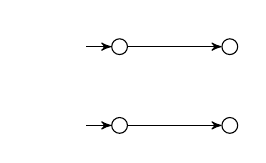
\begin{tikzpicture}[->, >=stealth', font=\footnotesize,
    state/.style={shape=circle, draw, initial text=,inner
      sep=.5mm,minimum size=2mm}, yscale=.5, xscale=.7]
    \node at (-1.5,0) {};
    \node at (-1.5,-2) {};
    \node[state, initial] (1) at (0,0) {};
    \node[state] (2) at (2,0) {};
    \node[state, initial] (3) at (0,-2) {};
    \node[state] (4) at (2,-2) {};
    \path (1) edge node[above]{} (2);
    \path (3) edge node[above]{} (4);
  \end{tikzpicture}
  \caption{\label{fi:conjvscomp}
    Two simple DMTS}
\end{figure}

Remark a subtle difference between conjunction and structural
composition, which we expose for discrete labels and CSP-style
composition: for the DMTS ,  shown in
Fig.~\ref{fi:conjvscomp}, both  and 
have only one state, but  and , so that  is inconsistent,
whereas  is not.

This definition extends the structural composition defined for modal
transition systems, with structured labels,
in~\cite{DBLP:journals/acta/FahrenbergL14}.  For DMTS specifications
(and hence also for -calculus expressions), the back translation
from \NAA to DMTS entails an exponential explosion.

\begin{theorem}
  \label{th:comp}
  Up to , the operator  is associative, commutative and
  monotone.
\end{theorem}

\begin{proof}Associativity and commutativity are clear by associativity and
  commutativity of .  Monotonicity is equivalent to the assertion
  that (up to )  distributes over the least upper bound
  ; one easily sees that for all specifications , ,
  , the identity is a two-sided modal refinement .  \qed
\end{proof}

\begin{corollary}[Independent implementability]
  \label{co:indimp}
  For all specifications , , , ,  and  imply .
  \noproof
\end{corollary}

\subsection{Quotient}
\label{se:quot}

Because of non-determinism, we have to use a power set construction for
the quotient, as opposed to conjunction and structural composition where
product is sufficient. For \NAA , , the quotient is , with  and .  States in  will be written .
Intuitively, this denotes that such state when composed with 
conforms to  for each ; we call this \emph{consistency} here.
 
We now define .  First, , so  is universal.  For any other state , its set of
\emph{permissible labels} is defined by

that is, a label is permissible iff it cannot violate consistency.  Here
we use the notation  as a shortcut for .

Now for each  and each , let
 be an enumeration of
all the possible states in  after an -transition.  Then we
define the set of all sets of possible assignments of next- states
from  to next- states from :

These are all possible next-state assignments which preserve
consistency.  Now let  and define

where , to
guarantee consistency no matter which element of , 
is composed with.

\begin{figure}\centering
  \begin{tikzpicture}[->, >=stealth', font=\footnotesize, xscale=2,
    yscale=1, state/.style={shape=circle, draw, initial text=,inner
      sep=.5mm,minimum size=3mm,initial distance=1.5ex}]
    \begin{scope}
      \node[state,initial] (s) at (0,0) {};
      \node[inner sep=0,outer sep=0] (ss) at (0.3,0){};
      \node[state] (s1) at (1.2,0.5) {};
      \path (s) edge[-] (ss);
      \path (ss)	edge [->,bend left] node[above]{}
      (s1);
      \node[state] (s2) at (1.2,-0.5) {};
      \path (ss)	edge [->,bend right]
      node[below]{}	(s2);
      \node (end) at (2,0.5) {};
      \path (s1) edge [->] node[above]{}	(end);
      \node (end2) at (2,-0.5) {};
      \path (s2) edge [->] node[below]{}	(end2);
    \end{scope}
    \begin{scope}[yshift=-20ex]
      \node[state,initial] (s) at (0,0) {};
      \node[state] (s1) at (1.2,0) {};
      \path (s)	edge [->] node[above]{}	(s1);
      \node (end) at (2,0) {};
      \path (s1)	edge [->,bend left] node[above]{}	(end);
      \path (s1)	edge [->, bend right] node[below]{}	(end);
      \path (s)  edge [->, bend right=80pt] node[below]{}  (end);
    \end{scope}
  \end{tikzpicture} 
  
  \bigskip

  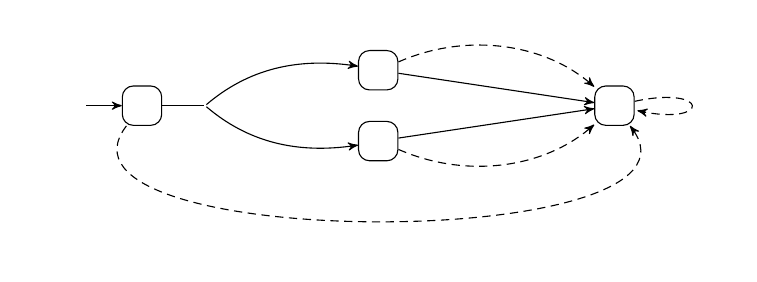
\begin{tikzpicture}[->, >=stealth', font=\footnotesize, xscale=2,
    yscale=1.5, state/.style={shape=circle,rectangle,rounded
      corners,draw,initial text=,inner sep=.5mm,minimum size=5mm,initial
      distance=1.5ex}]
    \begin{scope}
      \node[state,initial] (s) at (0,0) {};
      \node[inner sep=0,outer sep=0] (ss) at (0.4,0){};
      \node[state] (s1) at (1.5,0.3) {};
      \node[state] (s11) at (1.5,-0.3) {};
      \node[state] (s2) at (3,0) {};
      \path (s2) edge[loop right, densely dashed]
      node[above,pos=.2]{} (s2);
      \path (s) edge[-](ss);
      \path (ss) edge [->,bend left] node[above]{}  (s1);
      \path (ss) edge [->,bend right] node[below]{}  (s11);
      \path (s) edge [->,out=-90,in=-90,densely dashed,bend right=120pt]
      node[below]{} (s2);
      \path (s1)  edge [->,densely dashed, bend left=40pt]
      node[above]{} (s2);
      \path (s1)  edge [->] node[above]{} (s2);
      \path (s11)  edge [->,densely dashed, bend right=40pt]
      node[below]{} (s2);
      \path (s11)  edge [->] node[below]{} (s2);
    \end{scope}
  \end{tikzpicture} 
  \caption{\label{fi:quotientex}
    Two DMTS (top and center) and their quotient (bottom)}
\end{figure}

\begin{example}
  Fig.~\ref{fi:quotientex} shows two simple specifications and their
  quotient under , \ie~using addition of intervals for
  label synchronization (see Example~\ref{ex:composition}).  During
  the construction and the translation back to DMTS, many states were
  eliminated as they were inconsistent (their -set was
  empty). For instance, there is no may transition to state
  , because when it is composed with  there is no
  guarantee of a -transition, hence no guarantee to refine
  .

  Note that in order to have a finite representation of the quotient,
  we have to extend the label set to allow intervals which are not
  closed; for instance, the may-transition  from  to  comprises the fact
  that  for all  with .  This can be formalized by introducing a
  (partial) \emph{label quotient} operator  which is adjoint to label
  synchronization ,
  see~\cite{DBLP:journals/acta/FahrenbergL14}. \qed
\end{example}

\begin{theorem}
  \label{th:quotient-bool}
  For all specifications , , ,  iff .
\end{theorem}

\begin{proof}We show the proof for \NAA; for DMTS and -calculus expressions it
  will follow through the translations.  Let , , ; we show that  iff .

  We assume that the elements of  are pairwise disjoint
  for each ; this can be achieved by, if necessary,
  splitting states.

  First we note that by construction,  implies 
  for all .

  Assume that  and let  be the witnessing refinement relation.
  Let  (for
  readability, we abuse notation here and write 
  instead of ); we show that  is a witness for
  .

  Let  and .  Then
   with  and .  As , we can pair  with a set  such that .

  Let .  We show that :
  \begin{itemize}
  \item Let , then there are  with  and , .  By , there is  such that  and .  Note that
     is defined and .  Write .  By construction, there
    is an index  for which , hence .  Also, , hence  and consequently .
  \item Let , then there are 
    and  such that  and
    .  By , there is  for which  and .  Note
    that  is defined and .  Thus , and by , .
  \end{itemize}

  Assume, for the other direction of the proof, that  and let  (again
  abusing notation) be the witnessing refinement relation.  Define
   by
  
  we show that  is a witness for .  Let , with ,
  and .

  For every , write the set .  By assumption,  for , hence every  is contained in a unique .

  For every , let .  By , we have  such that .

  Now define
  
  We need to show that .

  Let  and ; we
  claim that .
  Let , then  for some  such that ,  and .  By disjointness,
  , hence by definition of ,  as was to be shown.

  For the reverse inclusion, let .  By
   and definition of ,
  there are  and  for
  which  and .  Thus , so that there must be  for
  which , but then also .

  We show that .
  \begin{itemize}
  \item Let .  For every  and
    every , we can use  and choose an element  for
    which  and .
    Let , then  and .
  \item Let , then we have 
    satisfying the conditions in~\eqref{eq:quotproof.M}.  Hence  for all , so that . \qed
  \end{itemize}
\end{proof}

\section{Robust Specification Theories}
\label{se:quant}

We proceed to lift the results of the previous sections to a
\emph{quantitative} setting, where the Boolean notions of modal and
thorough refinement are replaced by refinement \emph{distances}.  We
have shown in~\cite{DBLP:conf/fsttcs/FahrenbergLT11, DBLP:conf/aplas/FahrenbergL13,
  DBLP:conf/csr/BauerFLT12, DBLP:journals/tcs/FahrenbergL14,
  DBLP:journals/acta/FahrenbergL14} that a good setting for
quantitative analysis is given by the one of \emph{recursively
  specified trace distances} on an abstract commutative quantale as
defined below; we refer to the above-cited papers for a detailed
exposition of how this framework covers all common approaches to
quantitative analysis.

Denote by  the set of finite
and infinite traces over .

\subsection{Recursively specified trace distances}

Recall that a \emph{(commutative) quantale} consists of a complete
lattice  and a commutative, associative
addition operation  which distributes over arbitrary
suprema; we denote by ,  the bottom and top elements
of .  We call a function , for a set  and a
quantale , an \emph{-hemimetric} if it satisfies  for all  and  for all .

-hemimetrics are generalizations of distances: for  the extended real line, an -hemimetric is simply an extended hemimetric, \ie~a function
 which satisfies 
for all  and the triangle inequality  for all .  If  also is symmetric,
\ie~satisfies  for all , then  is
usually called a \emph{pseudometric}.  If  also satisfies the
principle of \emph{separability}, or indiscernibility of identicals,
\ie~such that  implies , it is called a
\emph{metric}.

A \emph{recursive trace distance specification}  consists of a quantale , a quantale morphism , an -hemimetric  (called \emph{lifted trace
  distance}), and a \emph{distance iterator} function .  For our purposes,  must be monotone in
the third and anti-monotone in the second coordinate and satisfy an
extended triangle inequality: for all  and , .

 is to specify  recursively in the sense that for all  and all  (and with ``''
denoting concatenation),

The \emph{trace distance} associated with such a distance specification
is  given by .

Note that  specializes to a distance on labels (because
); we require that this is compatible
with label refinement in the sense that  implies .  Then \eqref{eq:rec}~implies that whenever ,
then .  As an inverse
property, we say that  is \emph{recursively separating} if  implies that  and .

\begin{example}
  \label{ex:distances}
  We have shown in~\cite{DBLP:conf/fsttcs/FahrenbergLT11, DBLP:conf/csr/BauerFLT12,
    DBLP:conf/aplas/FahrenbergL13, DBLP:journals/tcs/FahrenbergL14,
    DBLP:journals/acta/FahrenbergL14} that all commonly used trace
  distances obey recursive characterizations as above.  We give a few
  examples, all of which are recursively separating, and refer
  to~\cite{DBLP:journals/tcs/FahrenbergL14,
    DBLP:journals/acta/FahrenbergL14} for further details:

  The \emph{point-wise} distance
  from~\cite{DBLP:journals/tcs/AlfaroFHMS05}, for example, has ,  and
  
  where  is a
  hemimetric on labels.  For the label set  from
  Example~\ref{ex:labelsets}, one useful example of such a hemimetric is
   if
   and  otherwise,
  \cf~\cite{DBLP:journals/fmsd/BauerFJLLT13}.

  The \emph{discounting} distance, also used
  in~\cite{DBLP:journals/tcs/AlfaroFHMS05}, again uses  and , but
  
  for a constant .

  For the \emph{limit-average} distance used
  in~\cite{DBLP:journals/tcs/CernyHR12} and other papers, , , and
  
  It is clear that limit-average distance has no recursive
  specification which uses  as for the
  other distances above.  Intuitively, the quantale  has to be used to memorize how many symbols one has
  seen in the sequences , .  This and other
  examples~\cite{DBLP:journals/tcs/FahrenbergL14,
    DBLP:journals/acta/FahrenbergL14} show that using general
  quantales in recursive trace distance specifications instead of
  simply  is necessary.

  The \emph{discrete} trace distance is given by 
  if  and  otherwise (here we have extended
   to traces in the obvious way).  It has a recursive
  characterization with , , and
   if  and
   otherwise. \qed
\end{example}

For the rest of this paper, we fix a recursively specified trace
distance.

\subsection{Refinement distances}

We lift the notions of modal refinement, for all our formalisms, to
distances.  Conceptually, this is done by replacing ``''
quantifiers by ``'' and ``'' by ``'' in the
definitions, and then using the distance iterator to introduce a
recursive functional whose least fixed point is the distance.

\begin{definition}
  \quad The \emph{lifted refinement distance} on the states of DMTS
    and  is the least fixed point to the equations
  
  for , .  For \NAA , , the right-hand side is
  replaced by
  
  and for -calculus expressions ,
   in normal form, it is
  
\end{definition}

Using Tarski's fixed point theorem, one easily sees that the lifted
refinement distances are indeed well-defined.  (Here one needs
monotonicity of  in the third coordinate, together with the fact that
 and  are monotonic.)

Note that we define the distances using \emph{least} fixed points, as
opposed to the \emph{greatest} fixed point definition of standard
refinement.  Informally, this is because our order is reversed: we are
not interested in maximizing refinement relations, but in
\emph{minimizing} refinement distance.

The lifted refinement distance between specifications is defined by

Analogously to thorough refinement, there is also a \emph{lifted
  thorough refinement distance}, given by  .

Using the  function, one gets distances 
and , with values in ,
which will be the ones one is interested in for concrete applications.

\begin{example}
  We compute the \emph{discounting} refinement distance between the DMTS
   and  in Figs.~\ref{fi:quantspecex1} and~\ref{fi:quantimp} on
  page~\pageref{fi:quantspecex1}, assuming sup-inf distance on
  quantitative labels (see Example~\ref{ex:distances}).  We have
  
  the least fixed point of which is seen to be .  Similarly, .  Note that  and . \qed
\end{example}

We recall the notion of \emph{refinement family}
from~\cite[Def.~6]{DBLP:journals/acta/FahrenbergL14} and extend it to
specifications.  We give the definition for \NAA only; for DMTS and
the modal -calculus it is similar.

\begin{definition}
  \label{de:reffam}
  A \emph{refinement family} from  to , for \NAA , , is an
  -indexed family of relations  with the property that for all  with , all , and all
  , there is  such that
  \begin{itemize}
  \item ,
  \item .
  \end{itemize}
\end{definition}

\begin{lemma}
  For all \NAA , , there exists a refinement family  from  to
   such that for all , there is 
  for which .
\end{lemma}

We say that a refinement family as in the lemma \emph{witnesses} .

\begin{proof}
  Define  by .  First, as  for all , , it
  is indeed the case that for all , there is  for which
  

  Now let  with  and .  Let .  We have , hence there is 
  such that
  
  But this entails that for all , there is  and  with , and that for all ,
  there is  and  such that
  . \qed
\end{proof}

The following quantitative extension of Theorems~\ref{th:dmtsvsaa-bool}
and~\ref{th:dmtsvsnu-bool} shows that our translations preserve and
reflect refinement distances.  Its proof is rather long and tedious,
hence we present it in a separate appendix to this paper.

\begin{theorem}
  \label{th:trans-moddist}
  For all DMTS , all \NAA ,  and all
  -calculus expressions , :
  
\end{theorem}

\subsection{Properties}

We sum up some important properties of our distances.

\begin{proposition}
  \label{pr:dist-prop}
  For all specifications , ,  implies
  , and  implies .  If  is recursively separating, then
   implies .
\end{proposition}

\begin{proof}We show the proposition for \NAA.  First, if , with
  , , then
  there is an initialized refinement relation , \ie~such that for all  and all , there is  for which
  \begin{itemize}
  \item  and
  \item .
  \end{itemize}
  Defining  by  for
  all , we see that  is an initialized refinement
  family which witnesses .

  We have shown that  implies .  Now if  instead, then for all
  , also , hence .

  To show the last property, assume  to be recursively separating.
  Define  by ; we show that  is a witness for .  By ,  is initialized.

  Let  and , then there is
   such that
  
  As  is recursively separating, we must have  in
  both these equations and .  But then , hence  is indeed a witness for . \qed
\end{proof}

\begin{proposition}
  \label{pr:dist-prop-hemi}
  The functions  and  are -hemi\-metrics, and ,
   are hemimetrics.
\end{proposition}

\begin{proof}
  We show the proof for \NAA.  The properties that  and  follow from
  proposition~\ref{pr:dist-prop}.

  We show the triangle inequality for .  The triangle inequality
  for  will then follow from standard arguments used to show that
  the Hausdorff metric satisfies the triangle inequality, see
  \eg~\cite[Lemma 3.72]{aliprantis2007infinite}.  Let , ,  be \NAA and ,  refinement families such that  and .

  Define  by
  
  We see that for all , there is  such
  that ; we show that  is a refinement family from
   to .

  Let  and , then we have
   and  such that
  ,  and .  Let , then we have  such that
  
  This in turn implies that there is  with
  

  Now let , then we get ,  and  as
  in~\eqref{eq:tri.1-2} and~\eqref{eq:tri.2-3}.  Let , then , and by the
  extended triangle inequality for , .

  Similarly, given , we can apply~\eqref{eq:tri.3-2}
  and~\eqref{eq:tri.2-1} to get  and 
  such that  and .

  We have shown that  and  are -hemimetrics.  Using
  monotonicity of the  function, it follows that  and 
  are hemimetrics.  \qed
\end{proof}

\begin{proposition}
  \label{pr:dist-prop.disc}
  For the \emph{discrete} distances,  if
   and  otherwise.  Similarly,  if  and  otherwise.
\end{proposition}

\begin{proof}We show the proposition for \NAA.  We already know that, also for the
  discrete distances,  implies 
  and that  implies .  We show
  that  implies .  Let  be a refinement
  family such that .  We show that  is a witness for ; it is clearly initialized.

  Let  and , then we have
   such that
  
  Using the definition of the distance, we see that the condition  is equivalent to  and ,
  hence~\eqref{eq:disctradistproof} degenerates to
  
  which are exactly the conditions for  to be a modal refinement.

  Again by definition, we see that for any \NAA , , either
   or , hence
   implies that .

  To show the last part of the proposition, we notice that
  
  Hence  if  and  otherwise.  \qed
\end{proof}

As a quantitative analogy to the implication from (Boolean) modal
refinement to thorough refinement (see Proposition~\ref{prop:mrtr}), the
next theorem shows that thorough refinement distance is bounded above by
modal refinement distance.  Note that for the discrete trace distance
(and using Proposition~\ref{pr:dist-prop.disc}), this is equivalent to
the Boolean statement.

\begin{theorem}
  \label{th:mdl-vs-tdl}
  For all specifications , , .
\end{theorem}

\begin{proof}We prove the statement for \NAA; for DMTS and -calculus
  expressions it then follows from Theorem~\ref{th:trans-moddist}.

  Let , .
  We have a refinement family  such that for all , there is
   with .
  Let , \ie~.

  Let  be an initialized modal refinement,
  and define a relation family  by .  We define a LTS  as follows:

  For all  with  and : We must have  with  and .  Then there is  such that
  \begin{itemize}
  \item for all , there is  with ,
  \item for all , there is  with .
  \end{itemize}
  This in turn implies that there is  satisfying
  the conditions in Definition~\ref{de:reffam}.  For all : add a transition  to .

  We show that the identity relation  is
  a witness for .  Let  and .  By construction, there is an  with , and for all , .

  We show that  is a witness for ; clearly,
   is initialized.  Let  with 
  and , then there is  with  and .  We also have  such that
  \begin{itemize}
  \item for all , there is  with ,
  \item for all , there is  with 
  \end{itemize}
  and thus  satisfying the conditions in
  Definition~\ref{de:reffam}.

  Let , then there is  with , hence also  and  with
   and .  But then , and 
  by construction.

  Let .  By construction, there is an  with .  This implies that there is
  ,  and  with
   and .
  But then there is also  with , hence
  . \qed
\end{proof}

\subsection{Disjunction and conjunction}

In order to generalize the properties of Theorem~\ref{th:condis} to our
quantitative setting, we introduce a notion of relaxed implementation
semantics:

\begin{definition}
  The \emph{-relaxed implementation semantics} of , for a
  specification  and , is
  
\end{definition}

Hence,  comprises all labeled transition systems which
are implementations of  \emph{up to }.  Note that by
Proposition~\ref{pr:dist-prop} and for  recursively separating,
.

\begin{theorem}
  \label{th:condis-q}
  For all specifications , ,  and ,
  \begin{itemize}
  \item ,
  \item ,
  \item , and
  \item .
  \end{itemize}
\end{theorem}

\begin{proof}We show the proof for DMTS.

  The proof that   is trivial: any refinement family
  witnessing  splits into two families
  witnessing  and  and vice
  versa.

  To show that  , let  be a
  witness for  and define  by
   for all .

  Let , then we have  so that , hence also .

  Let  and , then we have
   for which .  Assume first
  that , then there is 
  and  such that 
  and , hence .  By construction of , there are
   and  such that , but then by anti-monotonicity, .

  Now assume , then, by
  construction,\linebreak[4] .  Hence we have  such that .

  Let , then we have  and
   for which  and
  , hence .  By
  construction of , this implies that there are 
  and  such that , but then by
  anti-monotonicity, .

  We have shown that ; the proof of  is entirely analogous.

  The inclusion  is clear now: If , \ie~, then also  and , thus .

  To show that , one notices, like in the proof of
  Theorem~\ref{th:condis}, that for any LTS , any refinement family
  witnessing  or  is also a
  witness for  and vice versa. \qed
\end{proof}

The below example shows why the inclusions above cannot be replaced by
equalities.  To sum up, disjunction is quantitatively sound and
complete, whereas conjunction is only quantitatively sound.

\begin{figure}\centering
  \begin{tikzpicture}[->, >=stealth', font=\footnotesize,
    state/.style={shape=circle, draw, initial text=,inner
      sep=.5mm,minimum size=2mm}, yscale=1, xscale=1]
    \begin{scope}
      \node at (-1,0) {};
      \node[state, initial] (s) at (0,0) {};
      \node[state] (t) at (2,0) {};
      \path (s) edge node [below] {} (t);
    \end{scope}
    \begin{scope}[xshift=15em]
      \node at (-1,0) {};
      \node[state, initial] (s) at (0,0) {};
      \node[state] (t) at (2,0) {};
      \path (s) edge [densely dashed] node [below] {} (t);
    \end{scope}
    \begin{scope}[yshift=-10ex]
      \node at (-1,0) {};
      \node[state, initial] (s) at (0,0) {};
      \node[state] (t) at (2,0) {};
      \path (s) edge [densely dashed] node [below] {} (t);
    \end{scope}
    \begin{scope}[yshift=-10ex, xshift=15em]
      \node at (-1,0) {};
      \node[state, initial] (s) at (.5,0) {};
    \end{scope}
  \end{tikzpicture}
  \caption{\label{fi:ex-conj}
    LTS  together with DMTS ,  and their conjunction.
    For the point-wise or discounting distances, , but }
\end{figure}

\begin{example}
  \label{ex:no-qconj}
  For the point-wise or discounting distances, the DMTS in
  Fig.~\ref{fi:ex-conj} are such that  and , but .  Hence
  , and , but
  . \qed
\end{example}

\subsection{Structural composition and quotient}

We proceed to devise a quantitative generalization of the properties of
structural composition and quotient exposed in Section~\ref{se:specth}.
To this end, we need to use a \emph{uniform composition bound} on
labels:

Let  be a function which is monotone in both
coordinates, has 
and  for all
.  We require that for all  and  with  and ,  is
defined iff  is, and if both are defined, then


Note that \eqref{eq:synchbound}~implies that

Hence  provides a \emph{uniform bound} on distances between
synchronized labels, and \eqref{eq:synchbound} extends this property
so that it holds recursively.  Also, this is a generalization of the
condition that we imposed on  in Section~\ref{se:structlabels};
it is shown in~\cite[p.~18]{DBLP:journals/acta/FahrenbergL14} that it
holds for all common label synchronizations.

Remark that  can be understood as a (generalized) \emph{modulus of
  continuity}~\cite{encmath/continuity} for the partial function  given by label synchronization : with that notation, \eqref{eq:synchbound-s} asserts
that the distance from  to  is bounded by
 applied to the distance from  to .

The following theorems show that composition is uniformly continuous
(\ie~a quantitative generalization of independent implementability;
Corollary~\ref{co:indimp}) and that quotient preserves and reflects
refinement distance (a quantitative generalization of
Theorem~\ref{th:quotient-bool}).

\begin{theorem}\label{th:indimp-q}
  \quad For all specifications , , , , .
\end{theorem}

\begin{proof}We show the proof for \NAA.  For , let .  Let ,  be refinement families such that  and .  Define  by
  
  then it is clear that .  We
  show that  is a refinement family from  to .

  Let  and , then
  we have  with ,  and .  Let , then there must be ,  for which .  Thus we also have  and  such that
  

  Let , then .
  Let , then there are  and  for which .  Using~\eqref{eq:comp.1-3} and~\eqref{eq:comp.2-4}, we get ,  and 
  such that , , , and .

  Let  and , then we
  have .  Also,  and  imply that , and
  
  We have shown that for all , there
  exists  and  such
  that   and .  To show the reverse property,
  starting from an element , we can
  proceed entirely analogous,
  using~\eqref{eq:comp.3-1}\linebreak[4]and~\eqref{eq:comp.4-2}.  \qed
\end{proof}

\begin{theorem}
  \label{th:quot-q}
  For all specifications , , , we have .
\end{theorem}

\begin{proof}\quad We show the proof for \NAA.  Let  ,
  , ; we
  show that .

  We assume that the elements of  are pairwise disjoint
  for each ; this can be achieved by, if necessary,
  splitting states.

  Define  by .  (We again abuse notation and write
   instead of .)  We show that
   is a witness for .

  Let , then there is  for which it holds that , hence .

  Let ,  and .  Then 
  with  and .  As , we can pair  with an
  , \ie~such that the conditions in
  Definition~\ref{de:reffam} are satisfied.

  Let .  We show that the conditions in
  Definition~\ref{de:reffam} are satisfied for the pair :
  \begin{itemize}
  \item Let , then there are  with  and , .  Hence there is  and  such that  and
    .

    Note that  is defined and .  Write .  By construction, there is an index  for which
    , hence .  Also, , hence  and consequently .

  \item Let , then there are 
    and  such that  and .  Hence there are  and 
    for which  and .  Note that  is
    defined and .  Thus , and by , .
  \end{itemize}

  Assume, for the other direction of the proof, that .  Define  by
  
  we show that  is a witness for .

  Let .  We know that for every , there
  exists  such that .  By
  , we see
  that .

  Let  and ,
  with , and .

  For every , let us write .  By assumption,  for , hence every  is contained in a unique .

  For every , let .  By , we have  such that the
  conditions in Definition~\ref{de:reffam} hold for the pair .

  Now define
  
  We need to show that .

  Let  and ; we
  claim that .  Let , then 
  for some  such that ,  and .  By disjointness, , hence by definition of ,  as was
  to be shown.

  For the reverse inclusion, let .  By
  definition of , there are ,  and  for which  and .  Thus , so that
  there must be  for which , but then
  also .

  We show that the pair  satisfies the conditions of
  Definition~\ref{de:reffam}.
  \begin{itemize}
  \item Let .  For every  and every
    , we can use
    Definition~\ref{de:reffam} applied to the pair  to choose an
    element  and  for which
     and .  Let , then
     and .
  \item Let , then we have 
    satisfying the conditions in~\eqref{eq:quotproof2.M}.  Hence for all
    , there are , , , and  such that , 
    and\linebreak[4].  Let
    , then
     for all , hence . \qed
  \end{itemize}
\end{proof}

\section{Conclusion}

We have presented a framework for compositional and iterative design and
verification of systems which supports quantities and system and action
refinement.  Moreover, it is robust, in that it uses distances to
measure quantitative refinement and the operations preserve
distances.

The framework is very general.  It can be applied to a large variety of
quantities (energy, time, resource consumption etc.) and implement the
robustness notions associated with them.  It is also agnostic with
respect to the type of specifications used, as it applies equally to
behavioral and logical specifications.  This means that logical and
behavioral quantitative specifications can be freely combined in
quantitative system development.

As to future work, we believe that that the close relationship between
DMTS and the modal -calculus which we expose here should be helpful
for relating our robust semantics of the modal -calculus to other
quantitative logics~\cite{DBLP:conf/lics/HuthK97,
  DBLP:conf/fossacs/Mio11, DBLP:conf/concur/Alfaro03}.  We also plan to
implement the operations detailed here within the graphical tool
MoTraS~\cite{motras}.

\section*{Acknowledgements}

The second author acknowledges support by the European Research
Council (ERC) under grant 267989 (QUAREM), by the Austrian Science
Fund (FWF) under grants S11402-N23 (RiSE) and Z211-N23 (Wittgenstein
Award), the Czech Science Foundation Grant no.\ P202/12/G061, and the
People Programme (Marie Curie Actions) of the European Union's Seventh
Framework Programme (FP7/2007-2013) REA Grant no.\ 291734.  The first,
third and fourth authors acknowledge support by ANR MALTHY, grant
no.\ ANR-13-INSE-0003 from the French National Research Foundation, and
by the EU FP7 SENSATION project, grant no.\ 318490 (FP7-ICT-2011-8).

\begin{thebibliography}{10}

\bibitem{DBLP:journals/scp/AcetoFFIP13}
Luca Aceto, Ignacio F{\'a}bregas, David de~Frutos-Escrig, Anna
  Ing{\'o}lfsd{\'o}ttir, and Miguel Palomino.
\newblock On the specification of modal systems: A comparison of three
  frameworks.
\newblock {\em Sci. Comput. Program.}, 78(12):2468--2487, 2013.

\bibitem{books/AcetoILS07}
Luca Aceto, Anna Ing{\'o}lfsd{\'o}ttir, Kim~G. Larsen, and Ji{\v r}{\'i} Srba.
\newblock {\em Reactive Systems}.
\newblock {Cambridge Univ. Press}, 2007.

\bibitem{aliprantis2007infinite}
Charalambos~D. Aliprantis and Kim~C. Border.
\newblock {\em Infinite Dimensional Analysis: A Hitchhiker's Guide}.
\newblock {Springer-Verlag}, 2007.

\bibitem{DBLP:conf/fase/BauerDHLLNW12}
Sebastian~S. Bauer, Alexandre David, Rolf Hennicker, Kim~G. Larsen, Axel Legay,
  Ulrik Nyman, and Andrzej {W{\k a}sowski}.
\newblock Moving from specifications to contracts in component-based design.
\newblock In Juan de~Lara and Andrea Zisman, editors, {\em FASE}, volume 7212
  of {\em {Lect. Notes Comput. Sci.}}, pages 43--58. Springer, 2012.

\bibitem{DBLP:conf/mfcs/BauerFJLLT11}
Sebastian~S. Bauer, Uli Fahrenberg, Line Juhl, Kim~G. Larsen, Axel Legay, and
  Claus Thrane.
\newblock Quantitative refinement for weighted modal transition systems.
\newblock In Filip Murlak and Piotr Sankowski, editors, {\em MFCS}, volume 6907
  of {\em {Lect. Notes Comput. Sci.}}, pages 60--71. {Springer-Verlag}, 2011.

\bibitem{DBLP:journals/fmsd/BauerFJLLT13}
Sebastian~S. Bauer, Uli Fahrenberg, Line Juhl, Kim~G. Larsen, Axel Legay, and
  Claus Thrane.
\newblock Weighted modal transition systems.
\newblock {\em Form. Meth. Syst. Design}, 42(2):193--220, 2013.

\bibitem{DBLP:conf/csr/BauerFLT12}
Sebastian~S. Bauer, Uli Fahrenberg, Axel Legay, and Claus Thrane.
\newblock General quantitative specification theories with modalities.
\newblock In Edward~A. Hirsch, Juhani Karhum{\"a}ki, Arto Lepist{\"o}, and
  Michail Prilutskii, editors, {\em CSR}, volume 7353 of {\em {Lect. Notes
  Comput. Sci.}}, pages 18--30. {Springer-Verlag}, 2012.

\bibitem{DBLP:journals/mscs/BauerJLLS12}
Sebastian~S. Bauer, Line Juhl, Kim~G. Larsen, Axel Legay, and Ji{\v r}{\'i}
  Srba.
\newblock Extending modal transition systems with structured labels.
\newblock {\em Math. Struct. Comput. Sci.}, 22(4):581--617, 2012.

\bibitem{DBLP:conf/concur/Ben-DavidCU13}
Shoham Ben-David, Marsha Chechik, and Sebasti{\'a}n Uchitel.
\newblock Merging partial behaviour models with different vocabularies.
\newblock In Pedro~R. D'Argenio and Hern{\'a}n~C. Melgratti, editors, {\em
  CONCUR}, volume 8052 of {\em {Lect. Notes Comput. Sci.}}, pages 91--105.
  {Springer-Verlag}, 2013.

\bibitem{DBLP:conf/concur/BenesDFKL13}
Nikola Bene\v{s}, Beno\^{\i}t Delahaye, Uli Fahrenberg, Jan K{\v
  r}et{\'i}nsk{\'y}, and Axel Legay.
\newblock {H}ennessy-{M}ilner logic with greatest fixed points.
\newblock In Pedro~R. D'Argenio and Hern{\'a}n~C. Melgratti, editors, {\em
  CONCUR}, volume 8052 of {\em {Lect. Notes Comput. Sci.}}, pages 76--90.
  {Springer-Verlag}, 2013.

\bibitem{DBLP:journals/tcs/BenesKLS09}
Nikola Bene\v{s}, Jan K{\v r}et{\'i}nsk{\'y}, Kim~G. Larsen, and Ji{\v r}{\'i}
  Srba.
\newblock On determinism in modal transition systems.
\newblock {\em {Theor. Comput. Sci.}}, 410(41):4026--4043, 2009.

\bibitem{DBLP:conf/atva/BenesCK11}
Nikola Bene\v{s}, Ivana \v{C}ern{\'a}, and Jan K{\v r}et{\'i}nsk{\'y}.
\newblock Modal transition systems: Composition and {LTL} model checking.
\newblock In Tevfik Bultan and Pao-Ann Hsiung, editors, {\em ATVA}, volume 6996
  of {\em {Lect. Notes Comput. Sci.}}, pages 228--242. {Springer-Verlag}, 2011.

\bibitem{DBLP:journals/scp/BertrandLPR12}
Nathalie Bertrand, Axel Legay, Sophie Pinchinat, and Jean-Baptiste Raclet.
\newblock Modal event-clock specifications for timed component-based design.
\newblock {\em Sci. Comput. Program.}, 77(12):1212--1234, 2012.

\bibitem{DBLP:journals/tcs/BoudolL92}
G{\'e}rard Boudol and Kim~G. Larsen.
\newblock Graphical versus logical specifications.
\newblock {\em {Theor. Comput. Sci.}}, 106(1):3--20, 1992.

\bibitem{DBLP:journals/tcs/CaillaudDLLPW11}
Beno{\^{\i}}t Caillaud, Beno{\^{\i}}t Delahaye, Kim~G. Larsen, Axel Legay,
  Mikkel~L. Pedersen, and Andrzej W{\k a}sowski.
\newblock Constraint {M}arkov chains.
\newblock {\em {Theor. Comput. Sci.}}, 412(34):4373--4404, 2011.

\bibitem{DBLP:journals/iandc/CairesC03}
Lu{\'i}s Caires and Luca Cardelli.
\newblock A spatial logic for concurrency (part {I}).
\newblock {\em Inf. Comp.}, 186(2):194--235, 2003.

\bibitem{DBLP:conf/icalp/CardelliLM11}
Luca Cardelli, Kim~G. Larsen, and Radu Mardare.
\newblock Modular {M}arkovian logic.
\newblock In Luca Aceto, Monika Henzinger, and Ji{\v r}{\'\i} Sgall, editors,
  {\em ICALP (2)}, volume 6756 of {\em {Lect. Notes Comput. Sci.}}, pages
  380--391. {Springer-Verlag}, 2011.

\bibitem{DBLP:journals/sttt/DavidLLNTW15}
Alexandre David, Kim~G. Larsen, Axel Legay, Ulrik Nyman, Louis{-}Marie
  Traonouez, and Andrzej W{\k a}sowski.
\newblock Real-time specifications.
\newblock {\em {Int. J. Softw. Tools Techn. Transfer}}, 17(1):17--45, 2015.

\bibitem{DBLP:conf/concur/Alfaro03}
Luca de~Alfaro.
\newblock Quantitative verification and control via the mu-calculus.
\newblock In Roberto~M. Amadio and Denis Lugiez, editors, {\em CONCUR}, volume
  2761 of {\em {Lect. Notes Comput. Sci.}}, pages 102--126. {Springer-Verlag},
  2003.

\bibitem{DBLP:journals/tcs/AlfaroFHMS05}
Luca de~Alfaro, Marco Faella, Thomas~A. Henzinger, Rupak Majumdar, and
  Mari{\"e}lle Stoelinga.
\newblock Model checking discounted temporal properties.
\newblock {\em {Theor. Comput. Sci.}}, 345(1):139--170, 2005.

\bibitem{DBLP:journals/tse/AlfaroFS09}
Luca de~Alfaro, Marco Faella, and Mari{\"e}lle Stoelinga.
\newblock Linear and branching system metrics.
\newblock {\em IEEE Trans. Software Eng.}, 35(2):258--273, 2009.

\bibitem{DBLP:conf/sigsoft/AlfaroH01}
Luca de~Alfaro and Thomas~A. Henzinger.
\newblock Interface automata.
\newblock In {\em ESEC / SIGSOFT FSE}, pages 109--120. ACM, 2001.

\bibitem{DBLP:conf/emsoft/AlfaroHS02}
Luca de~Alfaro, Thomas~A. Henzinger, and Mari{\"{e}}lle Stoelinga.
\newblock Timed interfaces.
\newblock In Alberto~L. Sangiovanni{-}Vincentelli and Joseph Sifakis, editors,
  {\em EMSOFT}, volume 2491 of {\em {Lect. Notes Comput. Sci.}}, pages
  108--122. {Springer-Verlag}, 2002.

\bibitem{DBLP:journals/corr/abs-1212-4288}
Beno{\^{\i}}t Delahaye, Uli Fahrenberg, Kim~G. Larsen, and Axel Legay.
\newblock Refinement and difference for probabilistic automata.
\newblock {\em Logical Methods in Computer Science}, 10(3), 2014.

\bibitem{DBLP:journals/jlp/DelahayeLLPW12}
Beno{\^{\i}}t Delahaye, Kim~G. Larsen, Axel Legay, Mikkel~L. Pedersen, and
  Andrzej W{\k a}sowski.
\newblock Consistency and refinement for interval {M}arkov chains.
\newblock {\em J. Log. Algebr. Program.}, 81(3):209--226, 2012.

\bibitem{DBLP:journals/tcs/DesharnaisGJP04}
Josee Desharnais, Vineet Gupta, Radha Jagadeesan, and Prakash Panangaden.
\newblock Metrics for labelled {M}arkov processes.
\newblock {\em {Theor. Comput. Sci.}}, 318(3):323--354, 2004.

\bibitem{DBLP:conf/fase/FahrenbergALW14}
Uli Fahrenberg, Mathieu Acher, Axel Legay, and Andrzej W{\k a}sowski.
\newblock Sound merging and differencing for class diagrams.
\newblock In Stefania Gnesi and Arend Rensink, editors, {\em FASE}, volume 8411
  of {\em {Lect. Notes Comput. Sci.}}, pages 63--78. {Springer-Verlag}, 2014.

\bibitem{DBLP:journals/corr/abs-1207-4268}
Uli Fahrenberg and Axel Legay.
\newblock A robust specification theory for modal event-clock automata.
\newblock In Sebastian~S. Bauer and Jean{-}Baptiste Raclet, editors, {\em FIT},
  volume~87 of {\em EPTCS}, pages 5--16, 2012.

\bibitem{DBLP:conf/aplas/FahrenbergL13}
Uli Fahrenberg and Axel Legay.
\newblock Generalized quantitative analysis of metric transition systems.
\newblock In Chung{-}chieh Shan, editor, {\em APLAS}, volume 8301 of {\em
  {Lect. Notes Comput. Sci.}}, pages 192--208. {Springer-Verlag}, 2013.

\bibitem{DBLP:journals/acta/FahrenbergL14}
Uli Fahrenberg and Axel Legay.
\newblock General quantitative specification theories with modal transition
  systems.
\newblock {\em Acta Inf.}, 51(5):261--295, 2014.

\bibitem{DBLP:journals/tcs/FahrenbergL14}
Uli Fahrenberg and Axel Legay.
\newblock The quantitative linear-time--branch\-ing-time spectrum.
\newblock {\em {Theor. Comput. Sci.}}, 538:54--69, 2014.

\bibitem{DBLP:conf/fsttcs/FahrenbergLT11}
Uli Fahrenberg, Axel Legay, and Claus Thrane.
\newblock The quantitative linear-time--branching-time spectrum.
\newblock In Supratik Chakraborty and Amit Kumar, editors, {\em FSTTCS},
  volume~13 of {\em LIPIcs}, pages 103--114, 2011.

\bibitem{DBLP:conf/ictac/FahrenbergLT14}
Uli Fahrenberg, Axel Legay, and Louis-Marie Traonouez.
\newblock Structural refinement for the modal nu-calculus.
\newblock In Gabriel Ciobanu and Dominique M{\'{e}}ry, editors, {\em ICTAC},
  volume 8687 of {\em {Lect. Notes Comput. Sci.}}, pages 169--187.
  {Springer-Verlag}, 2014.

\bibitem{DBLP:conf/facs2/FahrenbergKLT14}
Ulrich Fahrenberg, Jan K{\v r}et{\'{\i}}nsk{\'{y}}, Axel Legay, and
  Louis{-}Marie Traonouez.
\newblock Compositionality for quantitative specifications.
\newblock In Ivan Lanese and Eric Madelaine, editors, {\em FACS}, volume 8997
  of {\em {Lect. Notes Comput. Sci.}}, pages 306--324. {Springer-Verlag}, 2014.

\bibitem{DBLP:journals/deds/FeuilladeP07}
Guillaume Feuillade and Sophie Pinchinat.
\newblock Modal specifications for the control theory of discrete event
  systems.
\newblock {\em Discrete Event Dynamic Systems}, 17(2):211--232, 2007.

\bibitem{DBLP:journals/tcs/Girard87}
Jean-Yves Girard.
\newblock Linear logic.
\newblock {\em {Theor. Comput. Sci.}}, 50:1--102, 1987.

\bibitem{DBLP:journals/jacm/Hennessy85}
Matthew Hennessy.
\newblock Acceptance trees.
\newblock {\em J. ACM}, 32(4):896--928, 1985.

\bibitem{DBLP:conf/formats/HenzingerMP05}
Thomas~A. Henzinger, Rupak Majumdar, and Vinayak~S. Prabhu.
\newblock Quantifying similarities between timed systems.
\newblock In Paul Pettersson and Wang Yi, editors, {\em FORMATS}, volume 3829
  of {\em {Lect. Notes Comput. Sci.}}, pages 226--241. {Springer-Verlag}, 2005.

\bibitem{DBLP:conf/fm/HenzingerS06}
Thomas~A. Henzinger and Joseph Sifakis.
\newblock The embedded systems design challenge.
\newblock In Jayadev Misra, Tobias Nipkow, and Emil Sekerinski, editors, {\em
  FM}, volume 4085 of {\em {Lect. Notes Comput. Sci.}}, pages 1--15.
  {Springer-Verlag}, 2006.

\bibitem{DBLP:conf/lics/HuthK97}
Michael Huth and Marta~Z. Kwiatkowska.
\newblock Quantitative analysis and model checking.
\newblock In {\em LICS}, pages 111--122. IEEE Computer Society, 1997.

\bibitem{DBLP:conf/fase/JacobsP01}
Bart Jacobs and Erik Poll.
\newblock A logic for the {J}ava modeling language {JML}.
\newblock In Heinrich Hu{\ss}mann, editor, {\em FASE}, volume 2029 of {\em
  {Lect. Notes Comput. Sci.}}, pages 284--299. {Springer-Verlag}, 2001.

\bibitem{DBLP:conf/lics/JonssonL91}
Bengt Jonsson and Kim~G. Larsen.
\newblock Specification and refinement of probabilistic processes.
\newblock In {\em LICS}, pages 266--277. IEEE Computer Society, 1991.

\bibitem{DBLP:journals/iandc/KlinS13}
Bartek Klin and Vladimiro Sassone.
\newblock Structural operational semantics for stochastic and weighted
  transition systems.
\newblock {\em Inf. Comput.}, 227:58--83, 2013.

\bibitem{DBLP:journals/tcs/Kozen83}
Dexter Kozen.
\newblock Results on the propositional -calculus.
\newblock {\em {Theor. Comput. Sci.}}, 27, 1983.

\bibitem{motras}
Jan K{\v r}et\'{\i}nsk{\'y} and Salomon Sickert.
\newblock {MoTraS}: A tool for modal transition systems and their extensions.
\newblock In Dang~Van Hung and Mizuhito Ogawa, editors, {\em ATVA}, volume 8172
  of {\em {Lect. Notes Comput. Sci.}}, pages 487--491. {Springer-Verlag}, 2013.

\bibitem{DBLP:journals/tcs/Larsen90}
Kim~G. Larsen.
\newblock Proof systems for satisfiability in {H}ennessy-{M}ilner logic with
  recursion.
\newblock {\em {Theor. Comput. Sci.}}, 72(2{\&}3):265--288, 1990.

\bibitem{DBLP:conf/formats/LarsenLTW11}
Kim~G. Larsen, Axel Legay, Louis-Marie Traonouez, and Andrzej W{\k a}sowski.
\newblock Robust specification of real time components.
\newblock In Uli Fahrenberg and Stavros Tripakis, editors, {\em FORMATS},
  volume 6919 of {\em {Lect. Notes Comput. Sci.}}, pages 129--144.
  {Springer-Verlag}, 2011.

\bibitem{DBLP:journals/tcs/LarsenLTW14}
Kim~G. Larsen, Axel Legay, Louis-Marie Traonouez, and Andrzej W{\k a}sowski.
\newblock Robust synthesis for real-time systems.
\newblock {\em {Theor. Comput. Sci.}}, 515:96--122, 2014.

\bibitem{DBLP:conf/mfcs/LarsenMP12}
Kim~G. Larsen, Radu Mardare, and Prakash Panangaden.
\newblock Taking it to the limit: Approximate reasoning for {M}arkov processes.
\newblock In Branislav Rovan, Vladimiro Sassone, and Peter Widmayer, editors,
  {\em MFCS}, volume 7464 of {\em {Lect. Notes Comput. Sci.}}, pages 681--692.
  {Springer-Verlag}, 2012.

\bibitem{DBLP:conf/lics/LarsenT88}
Kim~G. Larsen and Bent Thomsen.
\newblock A modal process logic.
\newblock In {\em LICS}, pages 203--210. IEEE Computer Society, 1988.

\bibitem{DBLP:conf/lics/LarsenX90}
Kim~G. Larsen and Liu Xinxin.
\newblock Equation solving using modal transition systems.
\newblock In {\em LICS}, pages 108--117. IEEE Computer Society, 1990.

\bibitem{DBLP:journals/toplas/LiskovW94}
Barbara Liskov and Jeannette~M. Wing.
\newblock A behavioral notion of subtyping.
\newblock {\em ACM Trans. Program. Lang. Syst.}, 16(6):1811--1841, 1994.

\bibitem{DBLP:conf/fossacs/Mio11}
Matteo Mio.
\newblock Probabilistic modal mu-calculus with independent product.
\newblock In Martin Hofmann, editor, {\em FOSSACS}, volume 6604 of {\em {Lect.
  Notes Comput. Sci.}}, pages 290--304. {Springer-Verlag}, 2011.

\bibitem{mu2}
Carroll Morgan and Annabelle McIver.
\newblock A probabilistic temporal calculus based on expectations.
\newblock In {\em Formal Methods Pathific}, 1997.

\bibitem{report/irisa/Raclet07}
Jean-Baptiste Raclet.
\newblock Residual for component specifications.
\newblock Publication interne 1843, IRISA, Rennes, 2007.

\bibitem{DBLP:conf/forte/Romero-HernandezF12}
David Romero-Hern{\'a}ndez and David de~Frutos-Escrig.
\newblock Defining distances for all process semantics.
\newblock In Holger Giese and Grigore Rosu, editors, {\em FMOODS/FORTE}, volume
  7273 of {\em {Lect. Notes Comput. Sci.}}, pages 169--185. {Springer-Verlag},
  2012.

\bibitem{DBLP:conf/wadt/Romero-HernandezF12}
David Romero-Hern{\'a}ndez and David de~Frutos-Escrig.
\newblock Distances between processes: A pure algebraic approach.
\newblock In Narciso Mart\'{\i}-Oliet and Miguel Palomino, editors, {\em WADT},
  volume 7841 of {\em {Lect. Notes Comput. Sci.}}, pages 265--282.
  {Springer-Verlag}, 2012.

\bibitem{DBLP:journals/cejcs/Sifakis11}
Joseph Sifakis.
\newblock A vision for computer science - the system perspective.
\newblock {\em Central Europ. J. Comput. Sci.}, 1(1):108--116, 2011.

\bibitem{DBLP:journals/corr/abs-1207-4269}
Louis-Marie Traonouez.
\newblock A parametric counterexample refinement approach for robust timed
  specifications.
\newblock In Sebastian~S. Bauer and Jean{-}Baptiste Raclet, editors, {\em FIT},
  volume~87 of {\em EPTCS}, pages 17--33, 2012.

\bibitem{DBLP:conf/sigsoft/UchitelC04}
Sebasti{\'a}n Uchitel and Marsha Chechik.
\newblock Merging partial behavioural models.
\newblock In Richard~N. Taylor and Matthew~B. Dwyer, editors, {\em SIGSOFT
  FSE}, pages 43--52. ACM, 2004.

\bibitem{DBLP:journals/tcs/BreugelW05}
Franck van Breugel and James Worrell.
\newblock A behavioural pseudometric for probabilistic transition systems.
\newblock {\em {Theor. Comput. Sci.}}, 331(1):115--142, 2005.

\bibitem{DBLP:journals/tcs/CernyHR12}
Pavol \v{C}ern{\'y}, Thomas~A. Henzinger, and Arjun Radhakrishna.
\newblock Simulation distances.
\newblock {\em {Theor. Comput. Sci.}}, 413(1):21--35, 2012.

\bibitem{encmath/continuity}
Continuity, modulus of.
\newblock Encyclopedia of Mathematics.
\newblock
  \url{http://www.encyclopediaofmath.org/index.php?title=Continuity,_modulus_of&oldid=30705}.

\end{thebibliography}


\section*{Appendix: Proof of Theorem~\ref{th:trans-moddist}}

  \noindent \underline{:}

  Let  and 
   be DMTS.  There exists a DMTS refinement family
   such that
  for all , there is  with .  We show that  is an \NAA
  refinement family.

  Let  and .  Let  and define
  
  The condition
  
  is satisfied by construction.  For the inverse condition, let , then , and as  is a DMTS
  refinement family, this implies that there is 
  and  for which  and , so that  by
  construction.

  We are left with showing that .  First we notice
  that by construction, indeed  for all .  Now let ; we need to show that .

  We have  such that .  We know that , so let .  Then there is  and  such that  and .  But  implies , hence .

  \medskip \noindent \underline{:}

  Let  and 
   be DMTS.  There exists an \NAA refinement family
   such that
  for all , there is  for which .  We show that  is
  a DMTS refinement family.  Let  and .

  Let , then we cannot have .
  Let , then
   by construction.  This implies that there is
  ,  and  such
  that  and , but then also  as was to be shown.

  Let  and assume, for the sake of contradiction, that
  there is no  for which  holds.  Then for each
  , there is an element 
  such that  does
  \emph{not} hold.

  Let , then  by construction.  Hence we have 
  such that .  Now , so let , then there is  and 
  such that  and , in contradiction to how  was
  constructed.

  \medskip \noindent \underline{:}

  Let ,  be
  \NAA, with DMTS translations 
  , .  There is
  an \NAA refinement family  such that for all , there is
   with .

  Define a relation family  by
  
  We show that  is a witness for .  Let  and
  .

  Let .  By construction of , there is  such that .  Then  implies that there must be
   and  such that  and .  Let
  , then .

  We show that : Let , then .  From  we get  such that
  
  hence ; also,  by
  construction of .

  Let , then we have  for which
   by construction of .  This in turn
  implies that there must be  such that .  By , we get  and  such that
   and .  Let , then
   and hence  for all .  By the same arguments as above, there is  for which .

  We miss to show that  is initialized.  Let , then
  we have  with .  As  is
  initialized, this entails that there is  with , which gives us  which satisfies the conditions in the definition of
  , whence .

  \pagebreak \noindent \underline{:}

  Let ,  be
  \NAA, with DMTS translations 
  , .  There is
  a DMTS refinement family  such that for all , there exists
   with .

  Define a relation family  by
  
  we will show that  is a witness for .

  Let ,  and , then by construction of , we have 
  with .

  Let  and define , then .  Now  implies that there must be  satisfying
  .  We have  such that ; we only miss to show that  for some  for which .  Let , then , hence there is  and  such that  and , but  also entails
  .

  Let  and define , then .  Now let , then , hence we have  and  such that  and .  By construction of
  , this implies that there is  with , and we have  for which .  Now if , then , hence there is  with , but  also
  gives .

  We miss to show that  is initialized.  Let  and
  .  As  is initialized, this gets us
   with , but  for some ,
  and then .

  \medskip \noindent \underline{:}

  Let  and
    be DMTS, with
  -calculus translations 
  and .  There is a DMTS
  refinement family
   such that
  for all , there exists  for which
  .

  Let , , , and
  .  Then , hence we
  have  and  with  and , but then
  also .

  Let , then also , so that
  there must be  such that , but then also .

  \medskip \noindent \underline{:}

  Let  and 
   be DMTS, with -calculus
  translations\linebreak[4] and .  There is a -calculus refinement family  such that for all
  , there exists  for which .

  Let  and , and assume that
  .  Then , so that
  there is ,  and  for which  and , but then also .

  Assume that , then .  Hence
  there is  so that , but then also .

  \medskip \noindent \underline{:}

  Let , 
  be -calculus expressions in normal form, with DMTS translations
   and .  There is a -calculus refinement
  family  such
  that for all , there is  for which .

  Let  and , and assume that
  .  Then , hence there
  are ,  and  such
  that  and , but then also .

  Assume that , then .  Hence
  there must be  such that , but then also
  .

  \medskip \noindent \underline{:}

  Let , 
  be -calculus expressions in normal form, with DMTS translations
   and .  There is a DMTS refinement family  such that for all
  , there is  for which .

  Let , , , and
  .  Then , hence we
  have  and  so that  and , but then
  also .

  Let , then also .  Hence we
  must have  with , but then also .  \qed

\end{document}
